
The passage of neutrons through matter is governed by the scattering of the neutrons off the various nuclei they encounter through the material.

The neutron flux is the average velocity of the neutrons within a certain volume

They are several nuclear interactions that are of interest for radiation portal monitors, of which several are presented in \autoref{tab:NeutronRxnProducts}.
\begin{table}
	\caption[Neutron Reactions and Reaction Energies]{Typically isotopes used in neutron radiation detectors}
	\label{tab:NeutronRxnProducts}
	\begin{tabular}{ c | c c c} 
		\toprule
		Reaction                           & Q-Value (MeV) & Thermal Cross Section & Application \\
		\midrule
		${}^3He + n \to p +{}^3H$          & 0.756     & 5,330 & Proportional counter gas \\
		${}^6Li + n \to {}^3H + \alpha$    & 4.78      & 940 & Lithium glass scintillators \\
		${}^{10}B + n \to \alpha + {}^7Li$ & 2.31      & 3,840 & Plastic scintillators \\
		${}^{157}Gd + n \to \gamma$        &various    & 259,000 & various \\
		\bottomrul
	\end{tabular}
\end{table}
The dependance of the cross section on the energy is shown in \autoref{fig:NeturonXS}.
The desire to thermalize the neutron flux (decreasing the average energy of the neutrons) is evident due to the dramatic increases of the cross sections for lower energies.
\begin{figure}
	\centering
	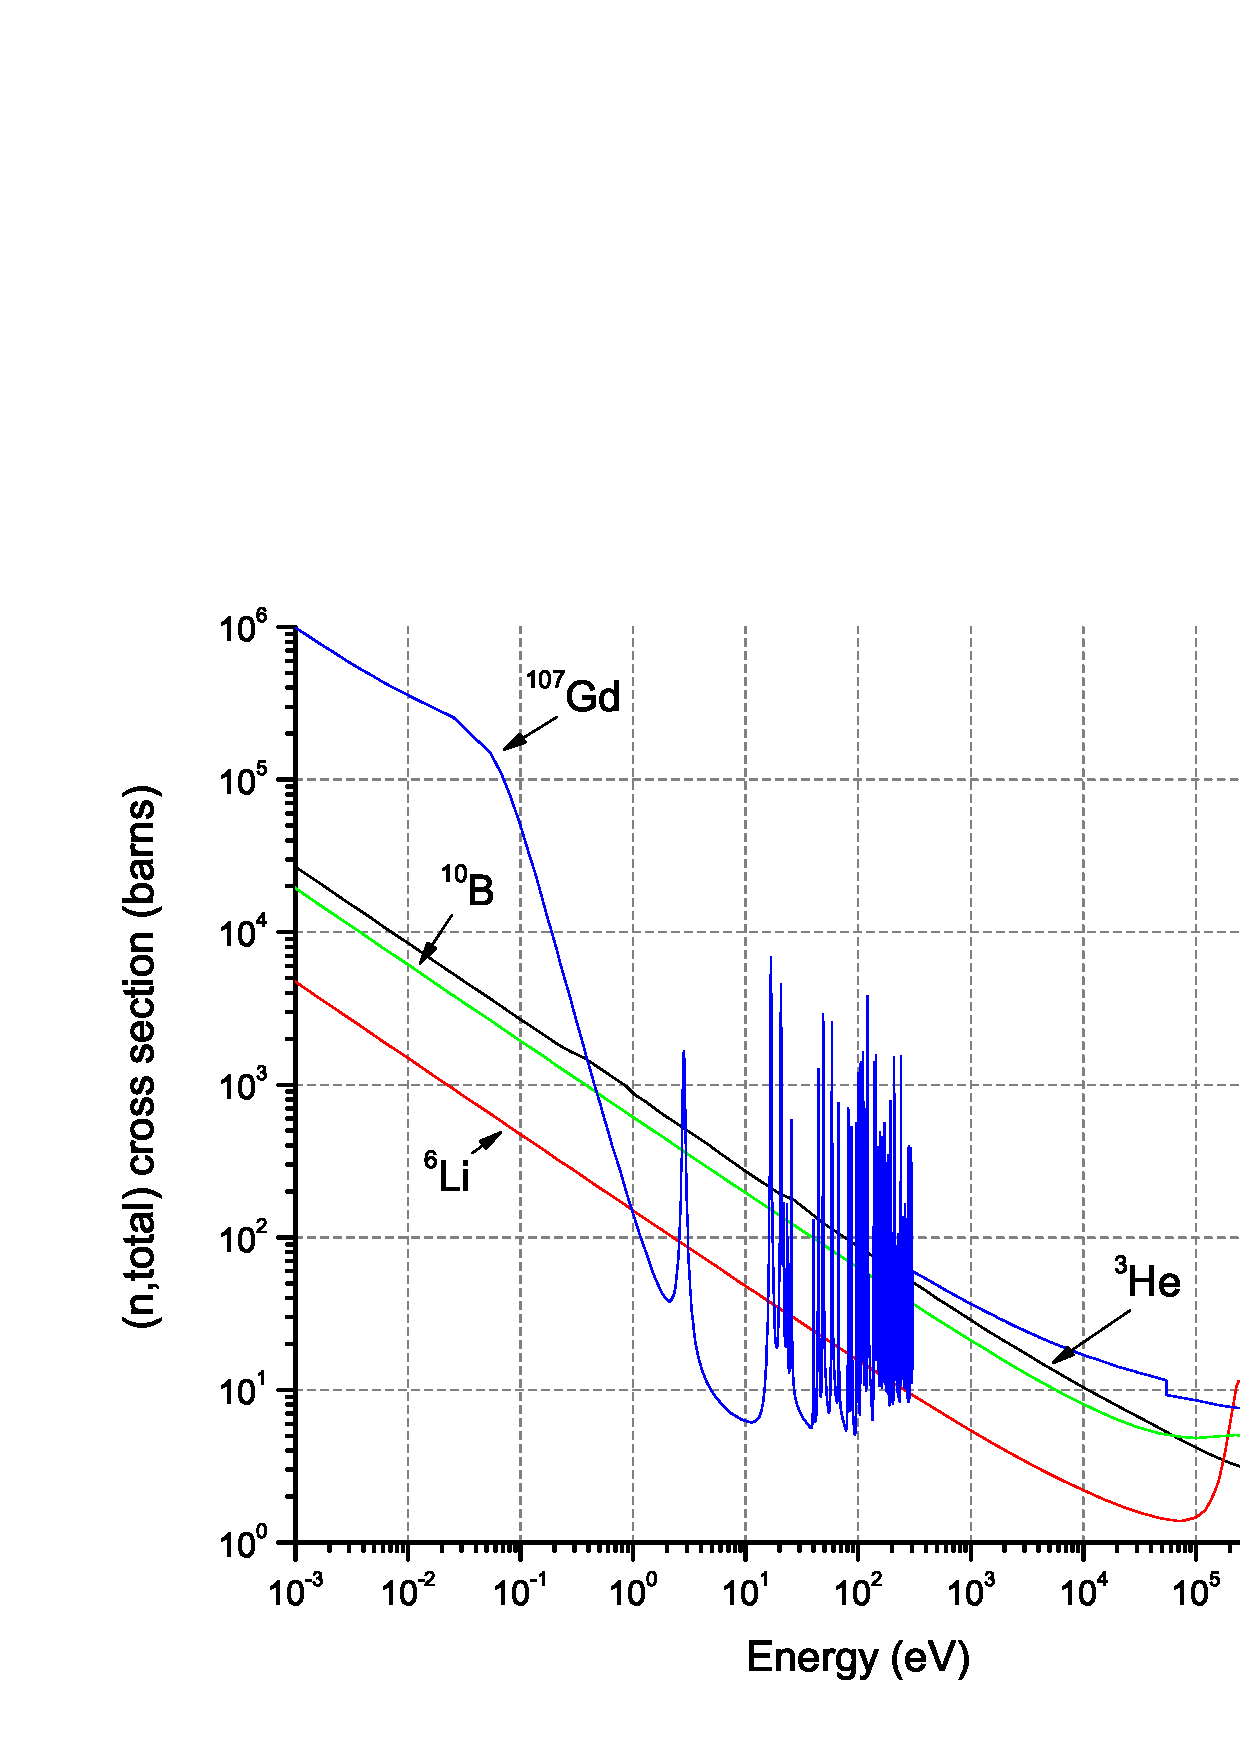
\includegraphics[width=\textwidth]{NeutronXS}
	\caption[Neutron Reaction Cross Sections]{Cross sections of typical isotopes used in neutron radiation detectors.  Neutrons at room temperature have an energy of \SI{0.025}{\ev}.}
	\label{fig:NeutronXS}
\end{figure}